\section{Google Analytics}

    \paragraph{}
    Google Analytics és un servei d'analítica web, proporcionat per Google, que s'encarrega de monitorar i reportar dades relatives al tràfic d'una aplicació web o aplicació mòbil.

    Mitjançant una implementació relativament simple, és possible emmagatzemar informació relativa a les pàgines visitades, la navegació entre pàgines, els sistemes operatius utilitzats, informació sobre els diferents navegadors, resolucions de pantalla, dispositius mòbils utilitzats i interaccions bàsiques dels usuaris amb les diferents pàgines del web.

    Gran part d'aquesta informació és capturada de forma automàtica, per Google Analytics, pel simple fet d'incloure el `snippet' de codi de l'eina a les nostres pàgines del domini web. A canvi, es disposa de moltes variables que poden ser creuades per tal d'analitzar el rendiment del domini web i l'ús que li donen els usuaris.

    De totes maneres, no s'espera que la nostra aplicació web disposi de grans quantitats de tràfic i la implementació de Google Analytics no ha vingut donada pel fet de poder analitzar el rendiment tècnic o d'usabilitat de l'aplicació, sinó per poder controlar el funcionament de la integració amb l'API de FamilySearch.

    Durant el desenvolupament de l'aplicació, mentre interactuàvem amb l'entorn sandbox de l'API, ens vàrem adonar que durant diversos dies i inclòs a vegades, períodes de tres o quatre dies, l'entorn no funcionava i les peticions llençades contra l'API eren cancel·lades.

    Per tal de poder monitorar en tot moment el funcionament de les interaccions dels usuaris amb l'API, s'ha utilitzat la funcionalitat de Google Analytics que permet enviar esdeveniments personalitzats, que o bé reflecteixen accions dels usuaris o condicions que s'han donat en l'aplicació web o mòbil.

    En concret, s'han creat quatre nivells d'esdeveniments diferents per cada una de les funcionalitats principals que interactuen amb l'API de FamilySearch:

    \begin{itemize}
        \item \emph{Formulari incorrecte:} En el cas que un usuari intenti llençar una petició contra l'API i aquesta no s'iniciï perquè el formulari contenia errors, es marca l'intent amb una etiqueta de formular incorrecte.
        \item \emph{Petició llençada:} Si la validació de tots els camps és correcta, s'envia un esdeveniment indicant que un intent de connexió amb l'API, s'ha llençat amb el SDK de FamilySearch i els paràmetres d'aquesta petició.
        \item \emph{Petició rebutjada:} En cas que el SDK no pugui resoldre la petició per qualsevol motiu, s'enregistra un esdeveniment que indica el rebuig de la petició i n'especifica el motiu (Per exemple, timeout, no existeix el recurs, excés de peticions en un període limitat de temps, etcètera).
        \item \emph{Petició retornada amb èxit:} Quan el SDK processa la petició i retorna resultats, s'envia un esdeveniment d'èxit.
    \end{itemize}

    Mitjançant l'existència d'aquests quatre nivells per cada una de les funcionalitats implementades, podrem conèixer l'estat de la connexió amb l'API de cada una d'elles, amb un esforç relativament baix.

    La figura~\ref{img:factsEvents} mostra els diferents quatre nivells d'esdeveniments per la funcionalitat evolució d'esdeveniments. Com es pot veure en la imatge, Google Analytics captura quantes vegades s'ha donat un esdeveniment concret en el període de temps definit i quantes sessions l'han contingut en algun moment donat.

    \begin{figure}
        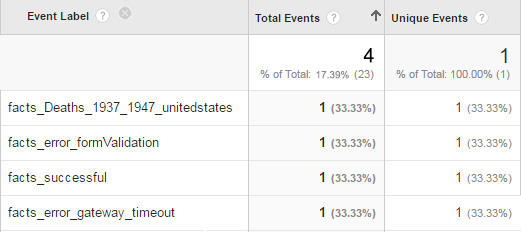
\includegraphics[scale=0.6]{10/04_factsEvents}
        \centering
        \caption{Exemple d'esdeveniments de la funcionalitat evolució d'esdeveniments}\label{img:factsEvents}
    \end{figure}

    A continuació, també citem els diferents exemples mostrats en la figura [] i hi afegim algun comentari.

    \begin{itemize}
        \item \textbf{Formulari incorrecte:} \emph{facts\_error\_formValidation}. Esdeveniment que s'envia quan la petició no s'ha arribat a processar perquè la configuració dels paràmetres no era correcta.
        \item \textbf{Petició llençada:} \emph{facts\_Deaths\_1937\_1947\_unitedstates}. Com es pot veure, quan es llança una petició contra l'API, també capturem el tipus d'esdeveniment cercat (defuncions), les dates per les quals s'ha cercat (1937-1947) i el país seleccionat (Estats Units).
        \item \textbf{Petició rebutjada:} \emph{facts\_error\_gateway\_timeout}. Aquest és un exemple dels esdeveniments que poden ser retornats quan l'API no ha pogut processar la petició.
        \item \textbf{Petició retornada amb èxit:} \emph{facts\_successful}. Esdeveniment que s'envia quan tot ha funcionat com s'esperava i l'API ha retornat resultats.
    \end{itemize}

    Els exemples d'esdeveniments anteriors, serveixen per demostrar el potencial que pot arribar a desencadenar una eina d'analítica web com Google Analytics.

    A part dels esdeveniments relatius a les funcionalitats implementades, que interactuen amb l'API de FamilySearch, també s'han implementat esdeveniments per controlar els intents d'identificació contra FamilySearch satisfactoris, les peticions de desconnexió, posicions dels exemples i propostes de projecte amb les que s'ha interactuat, interaccions amb la barra de navegació, posició de la persona seleccionada en la llista de resultats de la funcionalitat de cerca, etcètera.

    Tot i que el conjunt d'informació que s'ha exposat fins ara relativa a Google Analytics podria ser considerada simple, no creiem que sigui l'objectiu de la memòria entrar en molt més detall en les possibilitats d'una eina d'analítica web com aquesta, doncs realitzar una proposta profunda i exhaustiva de les possibilitats de monitoratge d'una web com la implementada, bé podria ser un projecte propi.
